\section{Transit Phenomenon \label{ss:transit}}

\begin{figure}[]
\begin{center}
	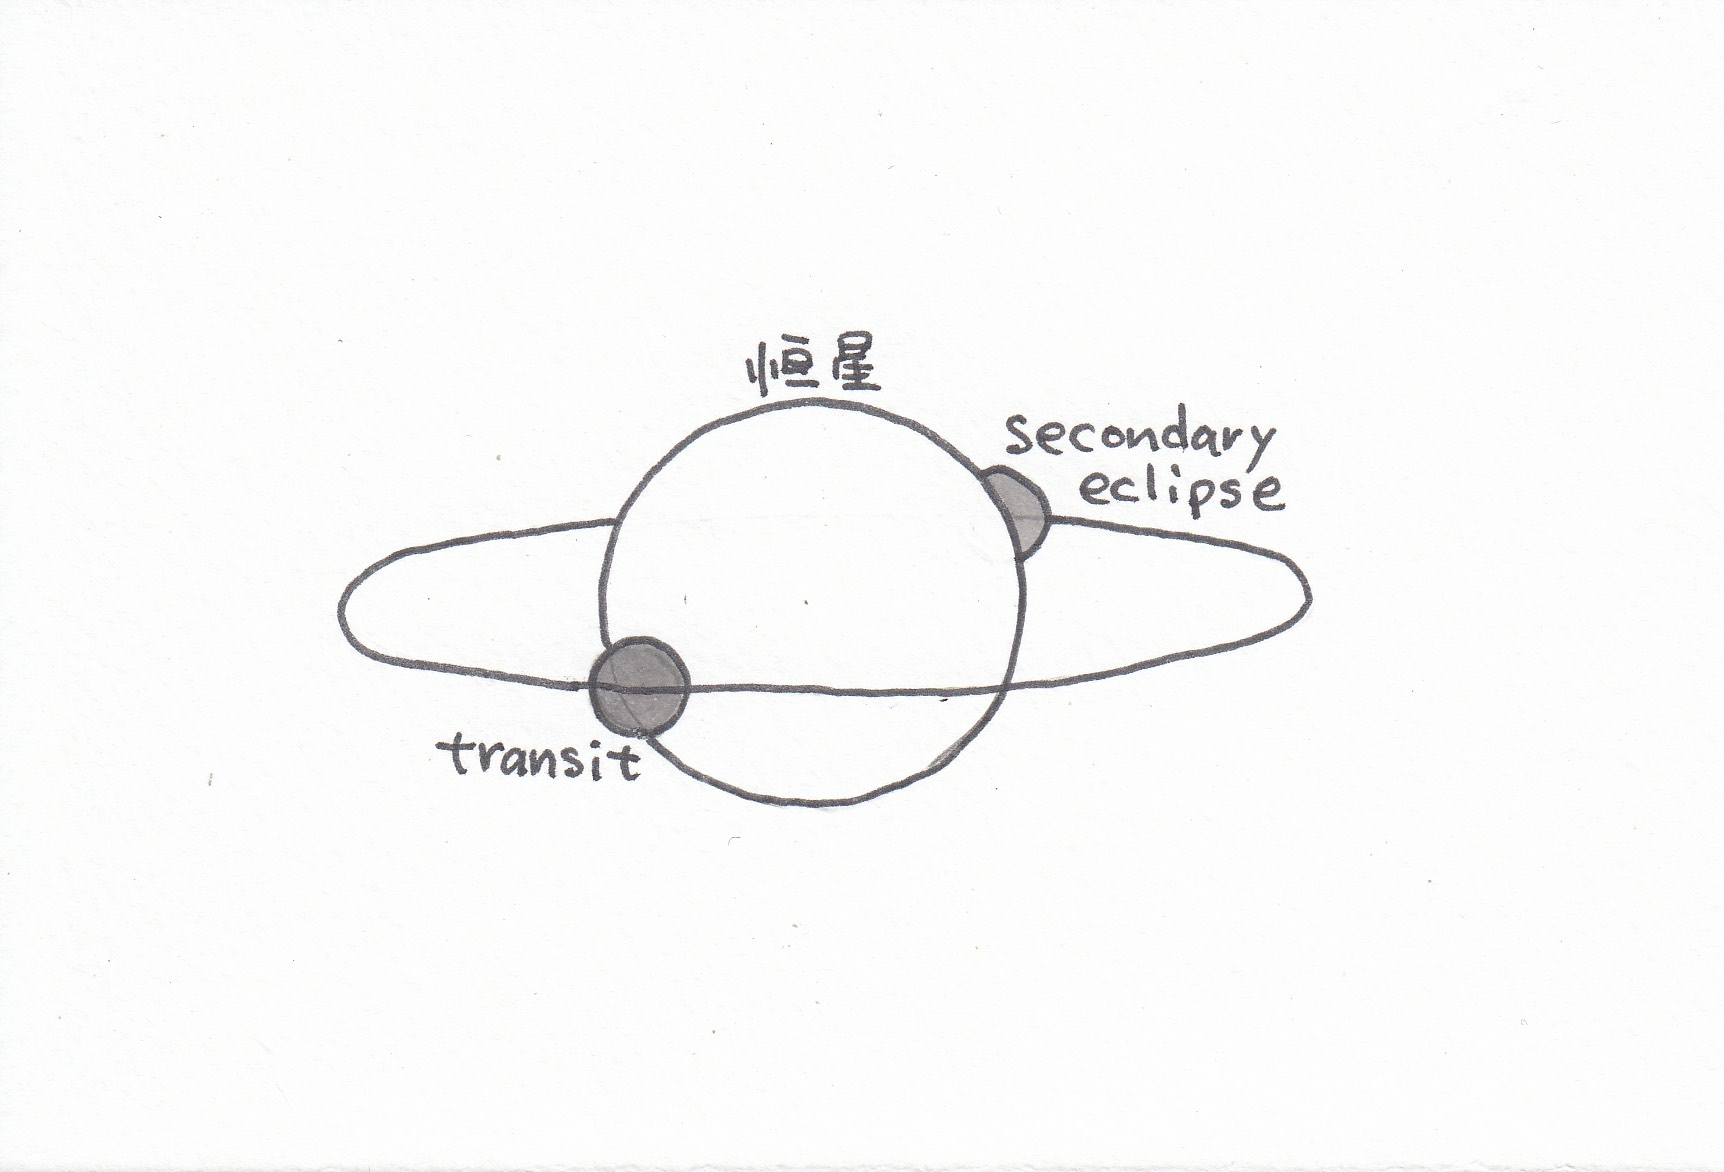
\includegraphics[width=\linewidth]{fig/transit.jpg}
	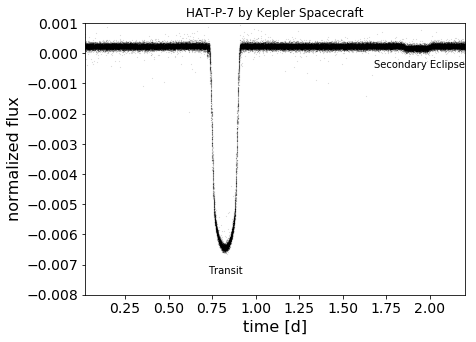
\includegraphics[width=\linewidth]{fig/Hatp7.png}
\end{center}
\caption{Schematic illustration of a transiting system (top) and an example of a transit light curve for the hot Jupiter HAT-P-7b, as observed by {\it Kepler} (bottom).\label{fig:hatp7b}}
\end{figure}

Variations in the stellar flux also contain signals due to the planet. The most straightforward example is the flux decrease caused by the shadow of the planet as it passes in front of the star, known as a {\bf transit dip}\index{とらんじっとげんこう@トランジット減光} (Fig.~\ref{fig:hatp7b}). In transiting systems, dimming is also observed when the planet passes behind the star. The latter is called the \textit{secondary eclipse}\index{にじしょく@二次食}\index{secondary eclipse@secondary eclipse} or simply \textit{occultation}\index{occlutation@occlutation}.  

The probability that a planet will transit, assuming a circular orbit and $R_p \ll R_\star$, corresponds to the region shown in Fig.~\ref{fig:transitprob}, and is given by
\begin{align}
p_\mathrm{tra} = \sin{(R_\star/a)} \sim \frac{R_\star}{a} = 0.005 \left(\frac{R_\star}{R_\odot}\right) \left(\frac{a}{1 \mathrm{\, au}}\right)^{-1},
\label{eq:tranp}
\end{align}
which yields about $0.5\%$ for a habitable-zone planet around a G-type star.  

\begin{figure}[!hbt]
\begin{center}
	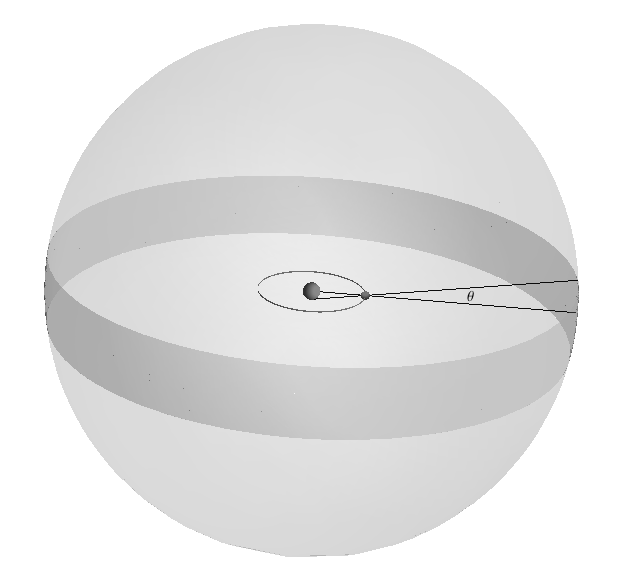
\includegraphics[width=\linewidth]{fig/transit_prob_bw.png}
\end{center}
\caption{Solid angle corresponding to lines of sight where the system appears transiting (shaded band). The star and planetary orbit are drawn inside. Since the radius of the outer sphere corresponds to the distance $d$ to the system, we can assume $a \ll d$. Thus, the probability that a random line of sight intersects the band is $4 \pi \sin{\theta}/ (4 \pi) \approx R_\star/a$.\label{fig:transitprob}}
\end{figure}

\subsection*{Transit Light Curve}

\begin{figure}[htb]
\begin{center}
	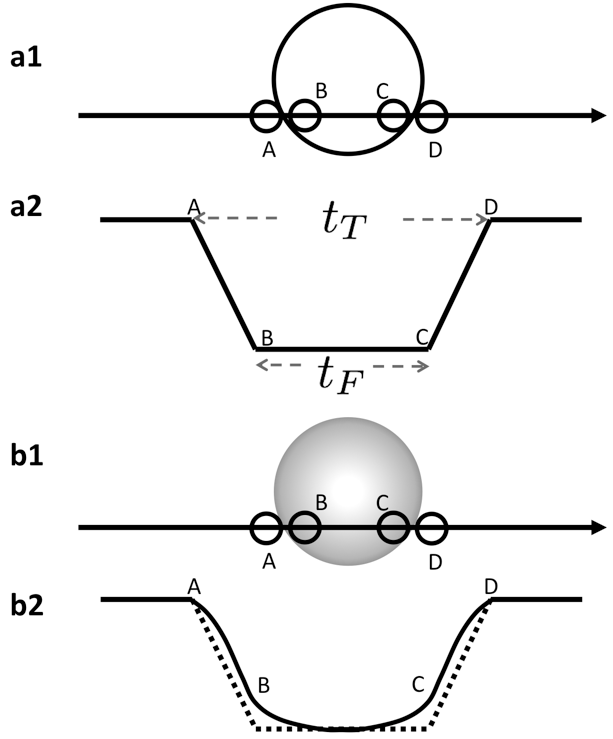
\includegraphics[width=\linewidth]{fig/transitmodel.png}
	\caption{Geometry of the transit light curve. Panel (a) shows the case of a uniformly bright star. In reality, stars exhibit limb darkening, producing the light curve shown in panel (b).}
	\label{fig:transitmodel}
\end{center}
\end{figure}

What physical quantities of an exoplanetary system can be inferred from a transit light curve?  
If multiple transits are observed, one can determine:  
\begin{itemize}
\item Orbital period $P$
\end{itemize}

The transit depth gives:
\begin{itemize}
\item The squared ratio of planetary to stellar radii, $k \equiv R_p/R_\star$
\end{itemize}

From the transit duration one can derive:
\begin{itemize}
\item The total transit duration $T_\mathrm{tot}$
\end{itemize}

More specifically, under the assumption of a uniformly bright star, one can also resolve ingress and egress phases, as illustrated in Fig.~\ref{fig:transitmodel}a. That is, the time between the start of ingress and the end of egress ($t_T$), as well as the time during which the planet is fully in front of the stellar disk ($t_F$), can be measured. In practice, since stars exhibit limb darkening, the actual light curve resembles Fig.~\ref{fig:transitmodel}b. By modeling limb darkening, $t_T$ and $t_F$ can still be estimated. A commonly used model is the quadratic limb-darkening law:
\begin{align}
I(\mu) = I(\mu=1) [ 1 - u_1 (1 - \mu) - u_2 (1 -\mu)^2],
\end{align}
where $\mu = \cos{\psi}$ and $\psi$ is the angle between the surface normal and the line of sight. Thus $\mu=1$ at the stellar disk center and $\mu=0$ at the limb. Note that integrating this model over the stellar disk yields $\pi R_\star^2 (1 - u_1/3 - u_2/6) I(\mu=1)$.  

Given $k$, one can also infer geometrically:
\begin{itemize}
\item The impact parameter: $b = \dfrac{a}{R_\star} \cos{i}$
\end{itemize}

With information on the stellar spectrum or stellar density $\rho_\star$, one can estimate $R_\star$ and $M_\star$. Knowing $P$, the semi-major axis $a$ can then be derived from Kepler’s third law, allowing the orbital inclination $i$ to be determined. If radial velocity measurements are available for the system, then $i$ yields the planetary mass $M_p$, and thus the planetary mean density
\begin{align}
\rho_p \equiv \frac{3 M_p}{4 \pi R_p^3}.
\end{align}
This makes it possible to classify exoplanets broadly.  

For circular orbits, the total duration is $T_\mathrm{tot} = 2 \sqrt{1-b^2} R_\star/v$, where $v$ is the planetary velocity. From Kepler’s third law neglecting planetary mass,
\begin{align}
P^2 = \frac{4 \pi^2}{G M_\star} a^3,
\end{align}
and noting $v=2 \pi a/P$, we obtain
\begin{align}
v^3=2 \pi G M_\star/P,
\end{align}
leading to $T_\mathrm{tot}^3 \propto P/\rho_\star$. Thus, with $P$ and $b$, the stellar density $\rho_\star$ can be determined from the transit duration.  

For a simple case with $b=0$, we have
\begin{align}
T_\mathrm{tot}  &= \left( \frac{3  P}{\pi^2 G \rho_\star} \right)^{1/3} \\
 &= 2.6 \mathrm{h} \left(\frac{P}{3 \mathrm{day}}\right)^{1/3} \left(\frac{\rho_\star}{\rho_\odot}\right)^{-1/3} \\
 &= 30  \mathrm{h} \left(\frac{P}{12 \mathrm{yr}}\right)^{1/3} \left(\frac{\rho_\star}{\rho_\odot}\right)^{-1/3}.
\end{align}
The second line corresponds to typical hot Jupiters, while the third line assumes Jupiter’s parameters. For longer periods of several years, transit durations exceed a day. For giant stars, lower stellar density also results in longer durations.  

\begin{itembox}{{\it column} -- Period and Light Curve Shape $\,^\dagger$}
%\tiny
\footnotesize
Assuming circular orbits, geometric considerations give
\begin{align}
\label{eq:totald}
\sin{ \left( \frac{\pi t_T}{P} \right)}  = \frac{R_*}{a} \sqrt{\frac{(1+k)^2 - b^2}{\sin^2{i}}}, \\
\label{eq:totalf}
\sin{ \left( \frac{\pi t_F}{P} \right)}  = \frac{R_*}{a} \sqrt{\frac{(1-k)^2 - b^2}{\sin^2{i}}},
\end{align}
and approximating $\sin{(\pi t_T/P)} \sim \pi t_T/P$ and $\sin{(\pi t_F/P)} \sim \pi t_F/P$, we obtain
\begin{align}
\label{eq:ra}
\frac{R_\star}{a} = \frac{\pi}{2 \sqrt{k}} \frac{\sqrt{t_T^2 - t_F^2}}{P} \sin{i}.
\end{align}
Using Kepler’s third law neglecting planetary mass,
\begin{align}
P^2 = \frac{4 \pi^2}{G M_\star} a^3,
\end{align}
and assuming $\sin{i} \sim 1$, we obtain
\begin{align}
\label{eq:pk}
P &= \frac{\pi G}{32} \frac{M_\star}{R_\star^3} \left( \frac{t_T^2 -t_F^2}{k} \right)^{\frac{3}{2}} \\
  &= \frac{\pi^2 G}{24} \rho_\star \left( \frac{t_T^2 -t_F^2}{k} \right)^{\frac{3}{2}}.
\end{align}
Thus, the only unknown quantity in the final expression is the stellar mean density $\rho_\star$, demonstrating that the stellar mean density can be inferred from transit light curve analysis.
\end{itembox}

\section{Transmission Spectroscopy}

Transmission spectroscopy measures the transit depth as a function of wavelength. Including wavelength dependence, the transit depth is expressed as
\begin{align}
\delta (\lambda) = \left( \frac{R_p(\lambda)}{R_\star} \right)^2,
\end{align}
where the wavelength dependence of the stellar radius is neglected. Here, $R_p(\lambda)$ corresponds to the effective planetary radius at the altitude where the atmosphere becomes opaque to stellar light. This altitude is determined by atomic and molecular absorption, scattering in the atmosphere, or by the solid planetary surface.  

Figure~\ref{fig:transmission} shows an example of transmission spectroscopy for a planet with a solid surface and a molecularly absorbing atmosphere. At wavelengths without molecular absorption, the solid surface defines $R_p$, while at wavelengths with absorption, the effective radius increases near the altitude where the optical depth becomes unity, causing a slightly deeper transit. Detecting such differences allows molecular species in the atmosphere to be identified.  

In this example, the continuum level was assumed to be set by the solid surface, but other cases include continua shaped by broad-band absorption, Rayleigh scattering, cloud scattering, the wings of strong absorption lines, or a pseudo-continuum formed by many weak lines.  

\begin{figure}[htb]
\begin{center}
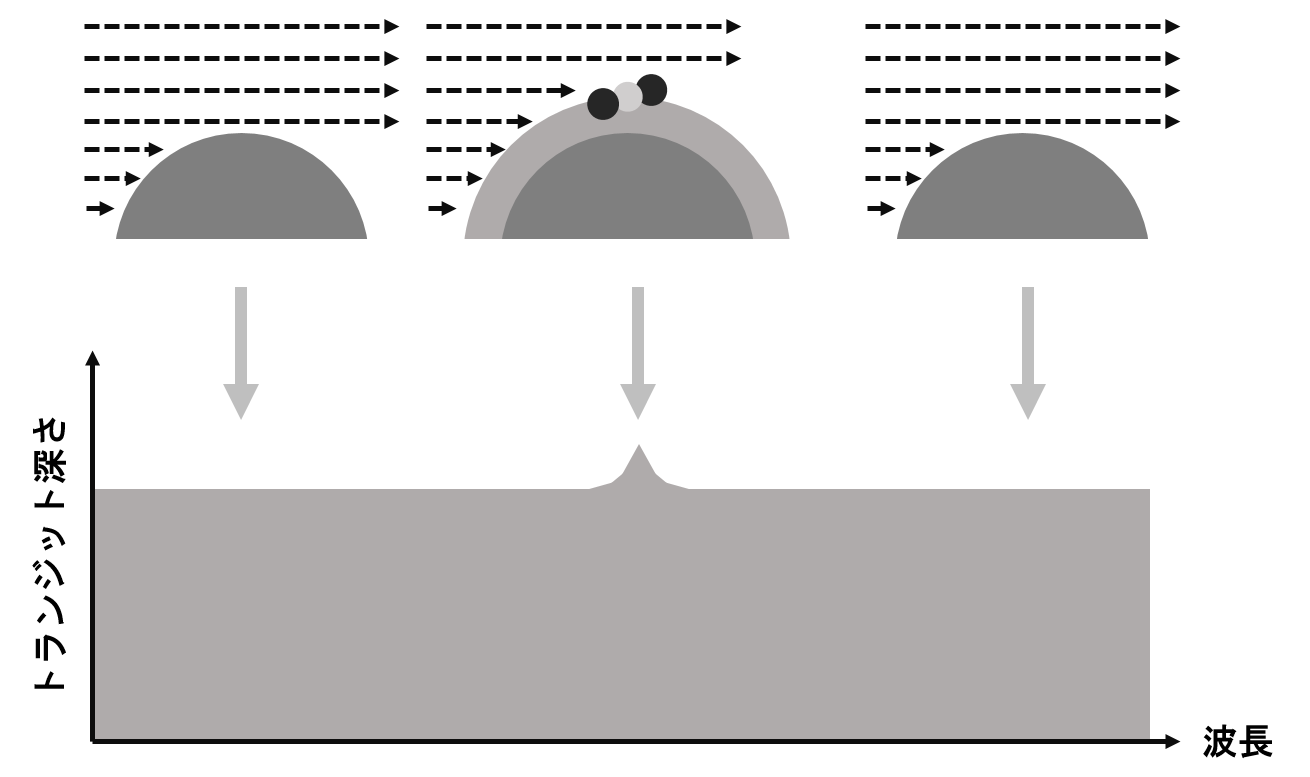
\includegraphics[width=\linewidth]{fig/transmission.png}
\caption{Schematic of transmission spectroscopy.\label{fig:transmission}}
\end{center}
\end{figure}

